\begin{refsection}

%************************************************
\chapter{Refinements to the model}
\label{ch:refined_model} %
%************************************************

{\sffamily\slshape The text in this chapter is identical to Section 3 of the published version of the preprint at \href{https://arxiv.org/abs/2504.10609}{arXiv:2504.10609} along with some additional figures.\\}

In this chapter, we develop an objective measure to rank pathways in a reaction network maximizing the probability of the entire pathway based on physical principles. 
Additionally, based on the notion that energy barriers of reactions are the determining factor for the kinetics of the network, we develop an automated methodology for computing such energy barriers, building on a combination of an array of existing computational tools. A key novelty is that in contrast to the standard manual intervention required to generate reaction trajectories from which the reaction barrier can be estimated, we try to automate this part of the process.
Lastly, we formulate an integer linear program which allows the user to specify queries for pathways in the network in a very flexible and generic way. Solving this integer linear program returns all pathways fulfilling the criteria, ranked by the objective measure mentioned above.
In short, this gives an automated, general, and flexible methodology for analyzing reaction networks, a methodology which offers a speed-up over manual search for pathways but with comparable quality.

In this chapter, we detail our proposed methodology for automating the search for kinetically informed pathways in reaction networks. As shown in Figure~\ref{fig: thermoEnergyBarrierCases}, the kinetics of the reaction can often lead to different results than those obtained from the reaction thermodynamics as done in Chapter~\ref{ch:thermodynamic_model}. In Sections~\ref{reaction_prob} and \ref{obj_func}, we first propose an objective function for ranking pathways in a reaction network annotated with kinetic data in the form of energy barriers for each reaction. In Section~\ref{implemented_model}, we then formulate an integer linear program (ILP) representing such networks and allowing the specification and execution of pathway searches. This part builds on the modeling described in Chapter~\ref{ch:thermodynamic_model}. We also describe how to search for not only one, but multiple solutions to a given pathway query, ordered by an objective function such as the one presented in Section~\ref{obj_func}. 

\newpage
\begin{figure}[!htb]
    \centering
    \begin{subfigure}{0.8\textwidth}
        \centering
        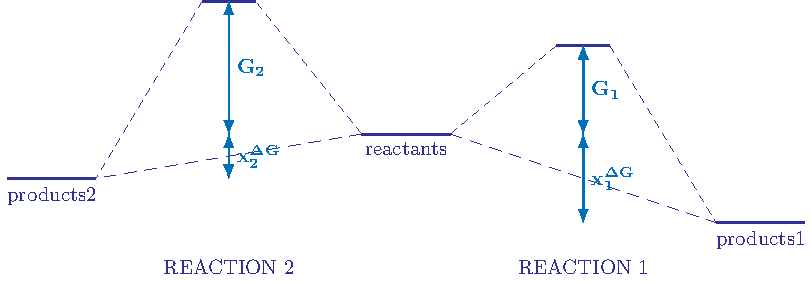
\includegraphics[width=\textwidth]{graphics/chapter4/case1.pdf}
        \caption{the thermodynamically more favored reaction are generally also kinetically preferred.}
        \label{fig: case1}
    \end{subfigure}
    \\
    \begin{subfigure}{0.8\textwidth}
        \centering
        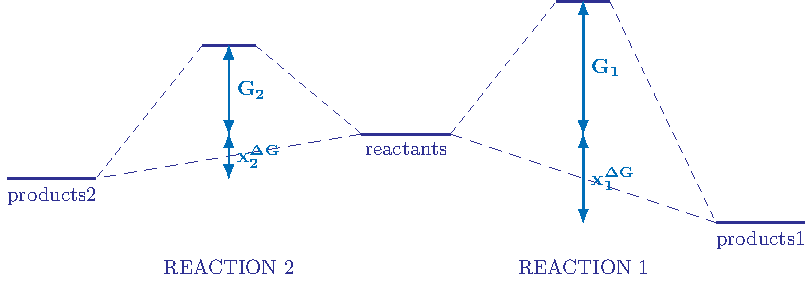
\includegraphics[width=\textwidth]{graphics/chapter4/case2.pdf}
        \caption{the thermodynamically less favored reaction with a smaller negative Gibbs free energy difference is also kinetically preferred because it has a lower energy barrier.}
        \label{fig: case2}
    \end{subfigure}
    \\
    \begin{subfigure}{0.8\textwidth}
        \centering
        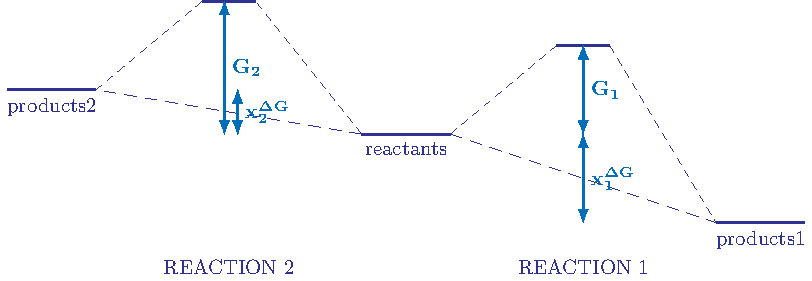
\includegraphics[width=\textwidth]{graphics/chapter4/case3.pdf}
        \caption{the thermodynamically unfavored reactions (with a positive Gibbs free energy difference) generally have higher energy barriers and are kinetically not preferred.}
        \label{fig: case3}
    \end{subfigure}
    \\
    \begin{subfigure}{0.8\textwidth}
        \centering
        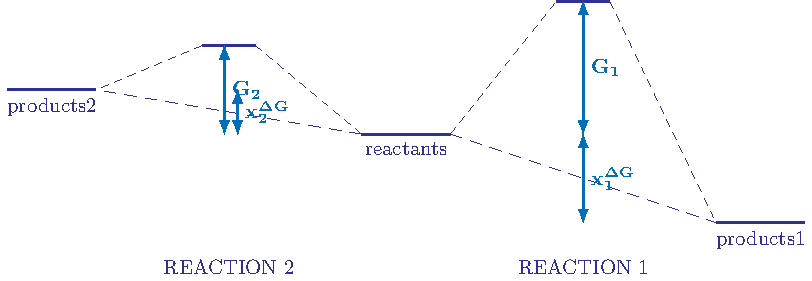
\includegraphics[width=\textwidth]{graphics/chapter4/case4.pdf}
        \caption{however, in fringe cases a thermodynamically unfavored reaction might have a lower energy barrier than a thermodynamically favored reaction.}
        \label{fig: case4}
    \end{subfigure}
    \vspace{0.2cm}
    \caption{Four of the many possible cases where the thermodynamics and kinetics of reactions might lead to different results. In cases \ref{fig: case2} and \ref{fig: case4}, the results based on thermodynamics are expected to be different from those obtained from kinetics.}
    \label{fig: thermoEnergyBarrierCases}
\end{figure}
\newpage


\section{From Rate Constants to Edge Weights}
\label{reaction_prob}

Irrespective of whether one uses Arrhenius' theory \cite{arrhenius1,arrhenius2}, collision theory or transition state theory \cite{eyring_equation}, the dependence of the rate constant~$k_e$ of a reaction~$e$ on the free energy barrier $G_e$ follows that of a negative exponential. The expression for the rate constant by Eyring's equation from transition state theory is
\begin{equation}
    k_e = \frac{k_b T}{h} \exp\left(-\frac{G_e}{RT}\right) \label{energy_barrier}
\end{equation}
where $R$ is the universal gas constant, $k_b$ is the Boltzmann constant, and $h$ is the Planck constant, each in their appropriate units.
In a well-stirred system where all the reactions in the reaction network are assumed to be concurrently taking place, the temperature can be considered to be the same for all reactions. Hence, it is not a factor affecting the relative rates of the reactions in the system.

Since our modeling is not aimed at capturing temporal changes in the concentrations of molecules, we make the simplifying assumption that all molecules in the reaction network are present with unit concentrations. 
This avoids the time propagation of the changes in the concentration of the molecules, as some of then a used up as reactants to produce other molecules.  
Under this assumption, the rate constant $k_e$ can be interpreted as being proportional to the probability of reaction~$e$ happening in a fixed small volume and time interval. 
A reaction with a higher rate constant (and lower energy barrier) is expected is occur more frequently, hence the probability of that reaction occurring in a fixed interval of time when a limited number of reactant molecules are present would be higher.
To interpret the rate constant as probabilities of the reaction in a given reaction network, we normalize these values to sum to one:
\begin{align}
    p(e) &= \frac{k_e}{\sum_{i\in E} k_i} \nonumber \\ 
    &= \frac{\frac{k_b T}{h} \exp\left(-\frac{G_e}{RT}\right)}{\sum_{i\in E} \frac{k_b T}{h} \exp\left(-\frac{G_i}{RT}\right)}\tag{\text{using }\ref{energy_barrier}} \\
    &= \frac{\frac{k_b T}{h} \exp\left(-\frac{G_e}{RT}\right)}{\frac{k_b T}{h} \sum_{i\in E} \exp\left(-\frac{G_i}{RT}\right)} \nonumber \\
    &= \frac{\exp\left(-\frac{G_e}{RT}\right)}{\sum_{i\in E} \exp\left(-\frac{G_i}{RT}\right)} \nonumber \\
    &= \frac{\exp\left(-\frac{G_e}{RT}\right)}{D} \label{prob_reaction}
\end{align}

Here, the denominator $\sum_{i\in E} \exp(-\frac{G_i}{RT})$ is the same for all reactions~$e$ and has been shortened to~$D$. In the current work, we assign the measure~$p(e)$ as the weight of the hyperedge representing~$e$ in an attempt to score reactions with lower energy barriers favourably.
However, the user is free to assign any other measures of weight to the hyperedges in the reaction network, if deemed better suited for a particular pathway search objective.

Figure~\ref{fig:twoReactions} tries to illustrate the reasoning behind assigning the weight measure to the respective reactions. There are two reactions with energy barriers $G_1$ and $G_2$ with $G_2 > G_1$ as shown in Figure~\ref{fig:two_reactions}. The energy distribution of the reactant molecules for both the reactions is given by the Maxwell-Boltzmann energy distribution in Figure~\ref{fig:boltzmannProfile}, and the fraction of molecules with the available energy to overcome the energy barrier of the respective reaction and form the products is given by
\begin{align*}
	f(N) &= \int_{G_i}^\infty P(E)\, dE \\
	&\sim \int_{G_i}^\infty \exp\left(-\frac{E}{RT}\right)\, dE \\
	&= \exp\left(-\frac{G_i}{RT}\right)
\end{align*}

\begin{figure}[!t]
    \centering
    \begin{subfigure}{0.9\textwidth}
        \centering
        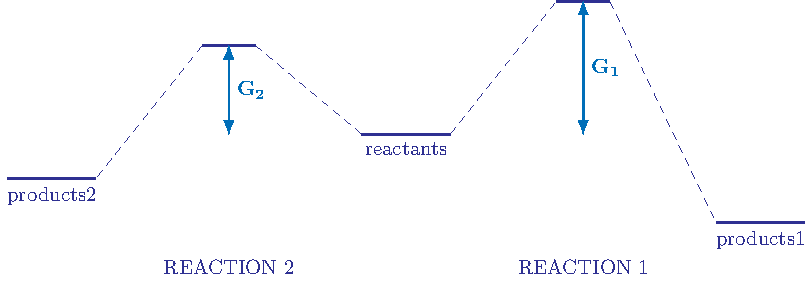
\includegraphics[width=\textwidth]{graphics/chapter4/twoReactions.pdf}
        \caption{Reactions with different energy barriers compete for the limited reactant molecules to form the respective products.}
        \label{fig:two_reactions}
    \end{subfigure}
    \vspace{0.5cm}
    \\
    \begin{subfigure}{0.9\textwidth}
        \centering
        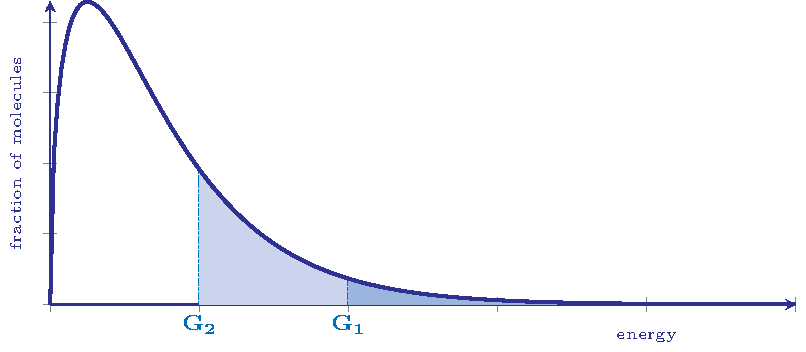
\includegraphics[width=\textwidth]{graphics/chapter4/twoReactionsNumberDensity.pdf}
        \caption{The reaction with the lower energy barrier is accessible to a larger fraction of the reactant molecules as more molecules have the energy required to form the products (denoted the shaded area under the curve).}
        \label{fig:boltzmannProfile}
    \end{subfigure}
    \caption{Of the two reactions competing for the same reactant molecules, the one with a lower energy barrier is favored as more reactant molecules can form the products. Therefore, it has a higher rate (given by Equation~\eqref{energy_barrier}) and assigned a higher probability of occurring by Equation~\eqref{prob_reaction} in a finite time with limited number of reactant molecules.}
    \label{fig:twoReactions}
\end{figure}

The rate of the reaction would be expected to be proportional to this fraction of molecules with enough energy to form the respective products, and might therefore, be used as a weight on a reaction to score its inclusion in the pathway. A pathway consisting of reactions with lower energy barriers would be scored higher as a larger fraction of molecules would overcome each reaction in the pathway. 

\section{Formulating an Objective Function}
\label{obj_func}

\begin{figure}[t]
    \centering
    \begin{subfigure}{\textwidth}
        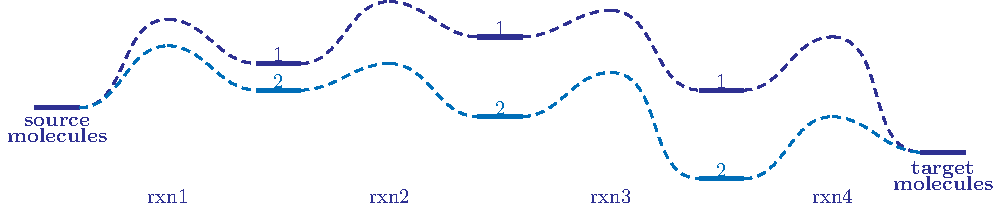
\includegraphics[scale=0.6]{graphics/chapter4/objFunc1.pdf}
        \caption{such a pathway 2 would be clearly more favored than pathway 1.}
        \label{fig: objFunc1}
    \end{subfigure}
    \vspace{0.2cm}
    \\
    \begin{subfigure}{\textwidth}
        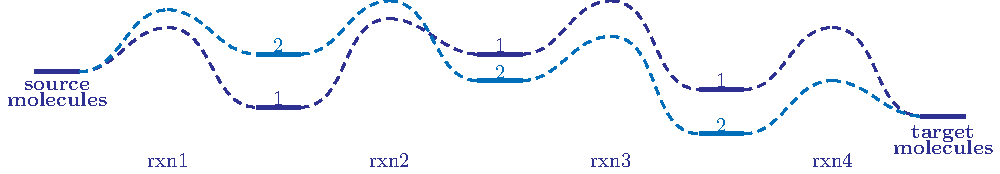
\includegraphics[scale=0.6]{graphics/chapter4/objFunc2.pdf}
        \caption{it is difficult to decide which of the pathways is more favored because not all molecules in one pathway have higher energies than the other (the energy profiles of the pathways cross at the second reaction).}
        \label{fig: objFunc2}
    \end{subfigure}
	\vspace{0.2cm}
    \\
    \begin{subfigure}{\textwidth}
        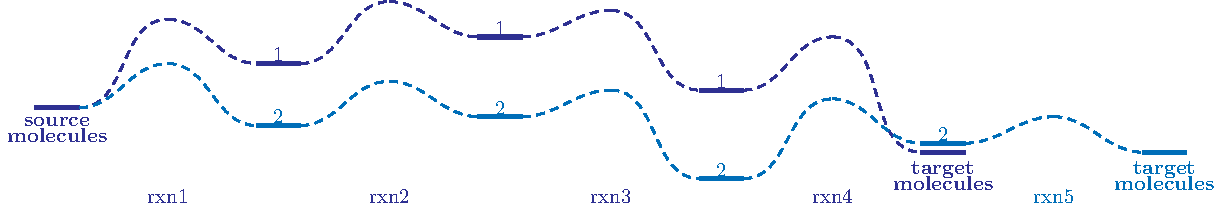
\includegraphics[scale=0.6]{graphics/chapter4/objFunc3.pdf}
        \caption{it is also difficult to decide if pathway 1 (a shorter pathway with $4$ reactions but higher barriers) is more favourable than pathway 2 (a longer pathway with $5$ reactions but lower barriers).}
        \label{fig: objFunc3}
    \end{subfigure}
    \caption{An objective function scores pathways and helps to decide which would be more favourable when it is not obvious such as in the cases depicted in~\ref{fig: objFunc2} and~\ref{fig: objFunc3}.}
    \label{fig: objFuncCases}
\end{figure}

We are interested in pathways from the given source molecules to the desired target molecule(s) that have a high overall probability of occurring in practice. This might not always be easy to determine when there are multiple pathways to the target molecule(s) as shown in Figure~\ref{fig: objFuncCases}. Considering individual reactions in a pathway as independent events (and abusing the notation~$e$ to mean the event of reaction~$e$ happening), the probability~$p_{\text{total}}$ of the entire set of reactions in the pathway occurring in one unit of time and one unit of volume is
\begin{align*}
    p_{\text{total}} &= p\left( \bigwedge_{e: f_e > 0} \left(e\wedge e \wedge \ldots f_e\text{ times}\right)\right) \\
    &= \prod_{e: f_e > 0} p(e)^{f_e} \\
    &= \prod_{e: f_e > 0} \left[\frac{\exp\left(-\frac{G_e}{RT}\right)}{D}\right]^{f_e} \tag{\text{using }\ref{prob_reaction}} \\
    &= \frac{\prod_{e: f_e > 0} \exp\left(-\frac{f_e\cdot G_e}{RT}\right)}{\prod_{e: f_e > 0} D^{f_e}} \\
    &= \left.\exp\left(-\frac{\sum_{e \in E} f_e\cdot G_e}{RT} \right) \middle/ D^{\sum_{e \in E} f_e}\right.
\end{align*}
Since the energy barrier $G_e$ is weighted by the flow $f_e$, the conditional sum $e: f_e > 0$ can be substituted by a simple sum over all hyperedges $e\in E$ because hyperedges with $f_e = 0$ do not contribute to the value of the sum.
The expression for the total probability of a pathway is a fraction and we take the logarithm of it to simplify it and make it a linear expression.
\begin{align*}
    \log p_{\text{total}} &= \log \left[\exp\left(-\frac{\sum_{e \in E} f_e\cdot G_e}{RT} \right) \middle/ D^{\sum_{e \in E} f_e}\right] \\
    &= -\frac{\sum_{e \in E} f_e\cdot G_e}{RT} - \left(\sum_{e \in E} f_e\right) \cdot \log D 
\end{align*}
The last line is proportional to the following expression obtained by multiplying by $RT$
\begin{equation*}
    -\sum_{e \in E} f_e\cdot G_e - RT\cdot \log D\cdot \sum_{e \in E} f_e
\end{equation*}
The probability of the set of reactions in the pathway is then maximized by maximizing the value of the obtained expression:
\begin{equation*}
    \max\left(-\sum_{e \in E} f_e\cdot \left(G_e + RT\cdot \log D \right)\right)
\end{equation*}
This is equivalent to the following minimization problem:
\begin{align}
    \min\left(\sum_{e \in E} f_e\cdot \left(G_e + RT\cdot \log D \right)\right) \label{proposed_objective}
\end{align}
This proposed objective value~\eqref{proposed_objective} is a linear expression because the $G_e$'s are constants from the input instance, $T$ is assumed constant, and $R$ is a physical constant. Also, the value $\log D = \log \left(\sum_{i\in E} \exp\left(-\frac{G_i}{RT}\right)\right)$ is constant when considering a fixed reaction network.

We note that via $D$, the objective value~\eqref{proposed_objective} of a pathway will depend on the underlying reaction network in which it is considered embedded. This may be regarded as a weakness. On the other hand, the objective value \eqref{proposed_objective} is intuitively appealing by being composed of two natural components: Its first component $\sum_{e \in E} f_e\cdot G_e$ favors pathways with small sums of energy barriers of the reactions in the pathway, weighted by the number of times it is used. Its second component $\sum_{e \in E} f_e \cdot \left( RT \, \log D\right)$ favors pathways with fewer reactions. The factor $ RT \log D$ can be viewed as weighting the relative importance of the two components and decides which of the two pathways is more favourable in cases such as the one shown in Figure~\ref{fig: objFunc3}.

\section{ILP Modeling} \label{implemented_model}

In this section, we express the modeling of Chapter~\ref{ch:toolbox} as an integer linear program (ILP). Recall the key idea that in a reaction network, pathways can be expressed as hyperflows and pathway queries can be expressed as constraints on hyperflows. Such constraints can simply be added to the ILP, after which the pathway queries can be executed by running an ILP-solver on the final ILP. We also describe how to search for multiple, structurally different solutions to a given pathway query, ordered by an objective function such as~\eqref{proposed_objective}.

Thus, in the ILP a pathway is represented by a vector of non-negative\footnote{Non-negative flow values require reversible reactions to be modeled as two separate hyperedges in the reaction network, but it also allows the flexibility to model some reactions as irreversible.} integer-valued variables~$f_e$, one variable for each reaction~$e$ in the reaction network. These flow variables are subject to the key constraint~\eqref{int_hyperflow_jakob}, as well as to the user-supplied constraints that specify the pathway query under consideration.

To model reversible reactions, separate hyperedges were added for the forward and backward directions of the reaction. This allows us to restrict the flows to non-negative integers only. The use of the reverse of a reaction would be denoted by a positive flow on the hyperedge in the opposite direction.
\begin{equation}
    f_e \geq 0 \tag{\ref{proposed_constraint2}}
\end{equation}

For each reaction~$e$, we add a boolean indicator variable $z_e$ which keeps track of whether the hyperedge~$e$ is used in the pathway or not. The values of these variables are assigned according to their respective flow variables following the biimplication constraints:
\begin{align}
    f_e = 0 &\iff z_e = 0 \tag{\ref{biimp3}} \\
    f_e \geq 1 &\iff z_e = 1 \tag{\ref{biimp4}}
\end{align}
We will use these indicator variables later when listing multiple, structurally different solutions to a given pathway query as elaborated in Section~\ref{enumerateSolutions} and for assigning a partial order to vertices in the pathway as elaborated in Section~\ref{partial_order}.\footnote{The indicator variables can also increase expressiveness when specifying pathway queries.} Many ILP solvers support addition of such indicator constraints \eqref{biimp1} and \eqref{biimp2} directly as implications to an ILP problem (which are then solved by a nonlinear, nonconvex reformulation of the indicator constraint). If this feature is not available, one can instead use the method of linearizing these implication constraints via a large constant~$M$.

\begin{table}[t]
    \centering
    \begin{scriptsize}
    \begin{tabular}{ccr}
        \toprule
        Constant & Datatype & Description \\
        \midrule
        $G_e$ & float & Weight of the hyperedge $e$ \\[1mm]
        $s_{ve}^+$ & integer & Count of molecule $v$ \\
        && on the LHS of a reaction $e$ \\[1mm]
        $s_{ve}^-$ & integer & Count of molecule $v$ \\
        && on the RHS of a reaction $e$ \\[1mm]
        $RT$ & float & Product of \\
        && universal gas constant \\
        && and temperature \\[1mm]
        $M$ & integer & Big integer used for \\
        && linearizing the constraints \\
        && (type promoted to float,\\
        && if required) \\
        \bottomrule
    \end{tabular}
    \end{scriptsize}
    \caption{Constants in the proposed ILP formulation.}
    \label{tab: ILP constants}
\end{table}%

\begin{table}[!h]
    \centering
    \begin{scriptsize}
    \begin{tabular}{ccr}
        \toprule
        ILP variable & Datatype & Description \\
        \midrule
        $f_e$ & integer & Flow variable for\\
        && a hyperedge $e$ \\
        && non-negative \\[1mm]
        $z_e$ & boolean & Indicator variable \\
        && denoting if a hyperedge \\
        && $e$ is used in the flow \\
        \bottomrule
    \end{tabular}
    \end{scriptsize}
    \caption{Variables in the proposed ILP formulation.}
    \label{tab: ILP variables}
\end{table}%

In summary, the resulting ILP looks as follows:

\begin{align}
    & \min\left(\sum_{e \in E} \left(f_e\cdot G_e + RT\cdot \log D\cdot f_e\right)\right) \tag{\ref{proposed_objective}} \\
    \forall e \in E\colon & 0 \leq f_e \tag{\ref{proposed_constraint2}} \\
    \forall v\in V \colon &\sum_{ e\in \overline{E} } s_{ve}^+ f_e - \sum_{ e\in \overline{E} } s_{ve}^- f_e = 0 \tag{\ref{int_hyperflow_jakob}}\\
    &\text{Constraints specifying the pathway query} \nonumber\\
    &\text{such as, inflow and outflow constraints} \nonumber\\
    & f_e = 0 \iff z_e = 0 \tag{\ref{biimp3}} \\
    & f_e \geq 1 \iff z_e = 1 \tag{\ref{biimp4}}
\end{align}

The constraints specifying the pathway consist of the desired outflow of the queried target molecule and the supplied source molecules. Additionally, it might involve constraints such an disallowing particular molecules as by-products (by restricting their outflow to zero), or disallowing the use of particular reactions (by specifying $f_e = 0 = z_e$ for those reactions). An overview of the variables and constants in the ILP can be found in Table \ref{tab: ILP variables} and \ref{tab: ILP constants}, respectively.

\subsection{Enumeration of solutions}
\label{enumerateSolutions}

\begin{figure}[t]
    \centering
    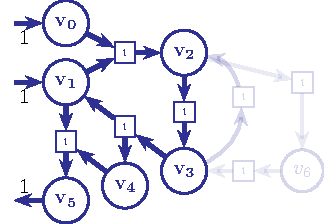
\includegraphics[scale=1.5]{graphics/chapter4/null_cycle.pdf}
    \caption{An example of a solution (the hyperflow of the entire figure) which contains a previous solution (the hyperflow shown in solid blue) as a subset, seen in terms of the edges (reactions) used. 
    Adding the faded hyperedges to the integer hyperflow depicted in solid blue creates a `null cycle' which creates a hyperflow solution that satisfies constraint~\eqref{int_hyperflow_jakob} but does not create a physically different solution.
    Addition of constrain~\eqref{subset_elimination} for all previously returned solutions ensures that such solutions are not returned.} 
    \label{fig: cover}
\end{figure}

We would like to enumerate multiple solutions to a pathway query in the reaction network. In this enumeration, we prefer to get a diverse set of pathways, in order to make the result more robust to uncertainties in the weights (i.e., the energy barrier values) assigned to the hyperedges. 
Such diversity offers a selection of alternative pathways for implementation, which is beneficial in case the single optimal solution turns out to be unattainable in practice (or just less desirable than expected due to circumstances not included in the modeling).
Some ILP solvers provide so-called solution pools which allow enumeration of solutions, but the process of populating this pool of solutions is often opaque.
More control is given in M{\O}D~\cite{mod_web}, which provides an option to enumerate multiple solutions based on a user-supplied specification of which subset of integer and binary variables to enumerate over~\cite{jakob_integer_hyperflows}.
For example, if the specification lists exactly the variables $z_e$ for each $e\in E$, then two pathways using the same set of hyperedges (but potentially with a difference in the flow value on some edges) will be considered equal,
and only the one with the best objective value is returned.
That is, if we define $supp(f) = \{e\in E \mid z_e = 1\}$ then two solutions $f_1$ and  $f_2$ are considered different exactly when $supp(f_1) \neq supp(f_2)$.

\begin{figure}[!h]
    \centering
    \begin{subfigure}{0.8\textwidth}
        \centering
        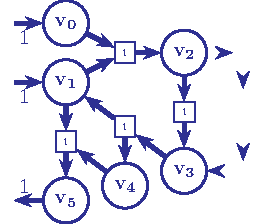
\includegraphics[scale=1.4]{graphics/chapter4/subset1.pdf}
        \vspace{0.5cm}
        \caption{An integer hyperflow solution with $4$ hyperedges.}
        \label{fig:solution1}
    \end{subfigure}
    \vspace{1cm}
    \\
    \begin{subfigure}{0.8\textwidth}
        \centering
        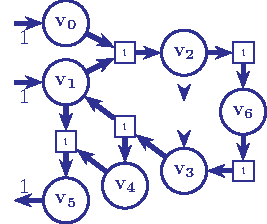
\includegraphics[scale=1.4]{graphics/chapter4/subset2.pdf}
        \vspace{0.5cm}
        \caption{Another integer hyperflow solution to the same flow query using $5$ hyperedges.}
        \label{fig:solution2}
    \end{subfigure}
    \vspace{1cm}
    \\
    \begin{subfigure}{0.8\textwidth}
        \centering
        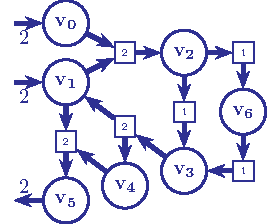
\includegraphics[scale=1.4]{graphics/chapter4/overlap.pdf}
        \vspace{0.5cm}
        \caption{An integer hyperflow satisfying all constraints listed in Section~\ref{implemented_model}. However, it is just the superposition of the solutions~\ref{fig:solution1} and~\ref{fig:solution2}.}
        \label{fig:overlap}
    \end{subfigure}
    \vspace{0.5cm}
    \caption{Addition of constrain~\eqref{subset_elimination} removes solutions like those shown in~\ref{fig:overlap} from the enumerated solutions.}
    \label{fig: union_solutions}
\end{figure}

However, in our case initial experimentation showed that using this enumeration policy, later enumerated solutions $f_2$ often contained a previous solution $f_1$, in the sense that $supp(f_1) \subsetneq supp(f_2)$, as exemplified in Figures~\ref{fig: cover} and~\ref{fig: union_solutions}.
To increase diversity of solutions, we opted for a custom enumeration scheme where $supp(f_2)$ of new solution~$f_2$ cannot contain $supp(f_1)$ of a previous solution~$f_1$ as a subset. When $supp(f_1) \subsetneq supp(f_2)$ holds for for a pair of solutions, the following statement must evaluate to \textsc{true} for the solution $f_1$:

\begin{center}
\begin{tabular}{lrl}
    & $\neg \bigwedge_{e\in supp(f_2)} z_e$ & $=$ TRUE\\
    or,& $\bigvee_{e\in supp(f_2)} \neg z_e$ & $=$ TRUE\\
    or,& $\sum_{e\in supp(f_2)} (1 - z_e)$ & $\geq 1$\\
    or,& $|supp(f_2)| - \sum_{e\in supp(f_2)} z_e$ & $\geq 1$\\
    or,& $\sum_{e\in supp(f_2)} z_e$ & $\leq |supp(f_2)| - 1$
\end{tabular}
\end{center}

In more detail: Let $f_i$ be the $i$th solution found. 
We then disallow subsequent solutions to contain $supp(f_i)$ by requiring that at least one of the hyperedges of~$f_i$ is not used. This is expressed via the following constraint:
\begin{equation}
    \sum_{e\in supp(f_i)} z_e \leq |supp(f_i)| - 1
    \label{subset_elimination}
\end{equation}
This constraint ensure that not all of the hyperedges in solution $f_i$ is used in some subsequent solution.
When the $k$th solution is to be found, there has thus been added $k-1$ of these constraints in total.
However, this method works only when the set of variables enumerated over is boolean, as is the case with $z_e$.

In Figure~\ref{fig: cover}, the hyperflow of the entire figure (with the part with lower opacity) has a subset of hyperedges which form a solution by itself. Therefore, $\bigwedge z_e$ evaluates to \texttt{TRUE} when evaluated over the set of hyperedges in the solution depicted in deep blue. Also, the left-hand side of the constraint~\ref{subset_elimination} is $\sum z_e = 4$ when evaluated over all the hyperedges in the hyperflow solution in dark blue which is $\nleq 4-1 = 3$. As a result, the hyperflow is not enumerated as a subsequent solution after the one in deep blue is added to the solution set.
Similarly the solution in Figure~\ref{fig:overlap}, would be excluded after either of the solutions in Figure~\ref{fig:solution1} or~\ref{fig:solution2} has been added to the solution set. The left-hand side of the constraint~\ref{subset_elimination} is $\sum z_e = 4$ when evaluated over all the hyperedges in the hyperflow in Figure~\ref{fig:solution1} which is $\nleq 4-1 = 3$. Therefore, the hyperflow in Figure~\ref{fig:overlap} is not enumerated as a subsequent solution after the one in Figure~\ref{fig:solution1} is added to the solution set. However, addition if the solution in Figure~\ref{fig:solution1} does not exclude the solution in~\ref{fig:solution2} as the left-side of constraint~\ref{subset_elimination} evaluates to $\sum z_e = 3$ (when summed over all hyperedges in the solution in Figure~\ref{fig:solution1}) which is $\leq 4-1 = 3$.

\subsection{Partial Ordering of Molecules}
\label{partial_order}

The ILP formulation of the problem~\cite{jakob_integer_hyperflows} accounts for the conservation of the for each molecule,
but not for temporal ordering of the reactions in the returned flow.
In scenarios such as synthesis planning~\cite{neurips_dag, rolf_synthesis_planning},
we would like to interpret a pathway as a directed acyclic process that generates the target molecule(s) unlike the one depicted in Figure~\ref{fig: selfLoop}.
We therefore introduce constraints to enforce a partial temporal order on the found pathways.

The ordering is implemented by introducing a supplementary integer variable $t_v$ for each vertex $v$ that keeps track of their ordering in the pathway.
The condition $t_{u} < t_{v}$ implies that the vertex $u$ is visited by the flow before the vertex $v$.
This is ensured by the following implication constraint:
\begin{align}
    \forall e\equiv (e^-, e^+)&\in E\colon \nonumber\\
        f_e &\geq 1 \implies t_v \geq t_u + 1, \label{prevent_back_edges}\\
        \forall &\text{ pairs } (u, v) \text{ such that } u \in e^-, v\in e^+ \nonumber
\end{align}

\begin{figure}[t]
    \centering
    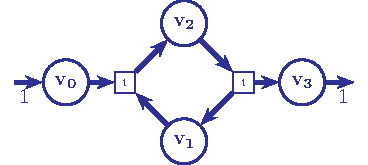
\includegraphics[scale=1.5]{graphics/chapter4/selfLoop.pdf}
    \caption{An example of a solution which satisfies the flow conservation constraint~\eqref{int_hyperflow_jakob} but cannot be realized if only $v_0$ is the allowed source and $v_3$ the requested target. To effect the first hyperedge, vertex $v_1$ is required to be present, which is in turn produced by the second hyperedge.
    Addition of constrain~\eqref{prevent_back_edges} remove such solution from being enumerated which are not physically realizable as a sequence of reaction to the target molecule(s).} 
    \label{fig: selfLoop}
\end{figure}

That is, the constraint ensures that reactants are assigned a lower order than products of a reaction with flow. 
We acknowledge that it can be too restrictive to enforce constraints to return pathways with an assigned partial ordering of vertices because they would eliminate all pathways with cycles in them.
Cycles are present whenever catalysts are used and in numerous metabolic networks.
We merely suggest the possibility of adding such constraints as part of the larger MILP model.
There might be other use cases where these partial constraints should be disabled in the model.
In these cases, the realizability question for pathways can be addressed using a separate,
more robust tool using the computationally more involved formalism of Petri nets on top of the MILP solver.
We refer the reader to a detailed study~\cite{sissel_realisability_petrinets} for a more thorough treatment of this issue of realizability of pathways.

\begin{figure}[!h]
    \centering
    \begin{subfigure}[b]{0.33\textwidth}
        \centering
        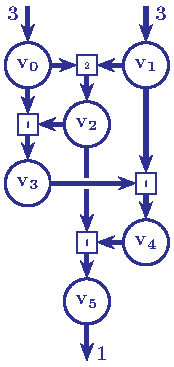
\includegraphics[scale=1.4]{graphics/chapter4/pathway_tvAssign.pdf}
    \end{subfigure}%
    \hspace{1cm}
    \begin{subfigure}[b]{0.5\textwidth}
        \centering
        \raisebox{3cm}{
		    \begin{tabular}{cc}
		    	\toprule
		    	vertex & $t_v$ \\
		   		\midrule
		    	$v_0$ & $0$ \\
		    	$v_1$ & $0$ \\
		    	$v_2$ & $1$ \\
		    	$v_3$ & $2$ \\
		    	$v_4$ & $3$ \\        
		    	$v_5$ & $5$ \\
		    	\bottomrule
			\end{tabular}
		}
    \end{subfigure}
    \caption{Addition of constrain~\eqref{linear_constraint8} ensures that the reactants are always available to effect a reaction either as products from a previous reaction or as sources. This prevents `back edges' in the pathway where are molecule is used that is produced later along the pathway.}
    \label{fig: partialOrderMolecules}
\end{figure}

The implication constraint in Equation~\eqref{prevent_back_edges} assigns the temporal ordering $t_v$ to each vertex $v$.
It is implemented as a linear constraint as
\begin{align}
    \forall \text{ pairs } (u, v)\,\,\,|\,\,\, \exists e\equiv (e^-, e^+) \text{ with } u &\in e^-, v \in e^+\colon \nonumber \\
    t_v - t_u - |V| (z_e - 1) - 1 &\geq 0 \label{linear_constraint8} \\
    \forall v\in V,\text{\hspace{1cm}}& \nonumber \\
    0 \leq t_v &\leq |V| \label{linear_constraint9}    
\end{align}
The constraint in Equation~\eqref{linear_constraint8} enforces the assignment $t_{v} > t_{u}$ only if the corresponding hyperedge is used in the hyperflow.
The size of the set of vertices in the hypergraph $|V|$ is used instead of the large integer $M$ in the constraint in Equation~\eqref{linear_constraint8} and as an upper bound for the temporal ordering variable $t_v$ for each vertex $v$ in the constraint in Equation~\eqref{linear_constraint9}.
The number of constraints added to the MILP model to determine the topological sorting of the vertices is $\mathcal{O}\left(|V|^2\right)$.

\section{Comparison with other methods}
\label{ch:discussions}

Previous work such as~\cite{shortest_path_hypergraph1,shortest_path_hypergraph2} have utilized hyperpaths in directed hypergraphs to depict pathways in reaction networks. However, they use the notion of path length to characterize the goodness of the pathway: a shorter pathway is considered better. Often this might not be the case as the shortest pathway might contain a slow or a high-cost reaction, which becomes a bottleneck for the entire pathway. Therefore, it is important to consider some physical attributes of the reactions (such as the barrier heights) in addition to the number of reactions while searching for pathways.

Most of previous work~\cite{graph_network1,graph_network2,graph_network3,heuristic_expert,reported_network} related to searching for pathways in reaction networks represent the underlying network as a graph with simple edges. However, this does not capture the nature of chemical reactions faithfully as it might involve multiple reactant molecules and produce multiple product molecules. Often the modeling tracks the most important molecules in the reactions~\cite{yaks,yarp}, relegating the other molecules involved in the reaction as reagents or side-products (in the style of synthesis maps of natural products). However, since the mathematical framework of hypergraphs exists to represent many-to-many mappings, we choose to use it instead of graphs. This has only one drawback: the visualization of the reaction networks becomes a little more involved and non-intuitive.

Studies focusing on large reaction networks such as~\cite{crn_expand_qm,shortest_path_hypergraph1,shortest_path_hypergraph2,reported_network} often extract the network from databases or existing knowledge. In contrast, using a generative methodology which can create the network on the fly (from a set of input molecules and a set of rules representing classes of reactions) allows us to investigate regions of the molecular space what have not been studied before. Moreover, it removes biases from previous experiments and studies that might have crept in while curating the database. If a particular promising molecule is not entered into the database, then no pathways queried from that network will contain it.

While there exists prior work which includes the generation of reaction networks, these networks were mostly generated using the gradient of potential information~\cite{iminoacetaldehyde2,yarp,empi1}. The determination of the gradient information used in potential energy surface explorations is computationally expensive and might limit the size of the studied network. Such studies focus on expanding the network only in the most promising directions and do not consider the remaining molecular space. Such a choice necessitated by computational costs hinders a thorough examination of the molecular space for pathways.  Chemical heuristics used by~\cite{yaks,heuristic_expert} offers a way out of this problem, and our method uses reaction templates to generate the networks this other studies in this class. We aim to generate an exhaustive network that is an over-approximation of what actually occurs in the system. The use of reaction templates allows us to cover all reaction possibilities in the generated network with a manageable computational cost. The current method uses graph rewriting and double pushouts as the formal framework behind the expansion of the network, which to the best of our knowledge is not used in other similar works.



\printbibliography[
  heading=subbibliography,
  title={References}
]

\end{refsection}
